\subsection{Grundlagen}

In diesem Abschnitt wird der Raum $\mathbb{R}^2$ anstatt der unter~\ref{subsec:voronoi-introduction} eingeführte Raum $\mathbb{R}^m$ verwendet, da die Komplexität ansonsten die Beispiele unnötig verkomplizieren würde. Es handelt sich dabei also um die euklidische Ebene.

Gegeben sei eine finite Punktemenge $O$ bestehend aus zwei oder mehr Elementen der euklidischen Ebene $\mathbb{R}^2$. Es werden nun alle Orte dieses Raumes dem nächsten Punkt $p = \{p_x, p_y\}$ der Punktemenge $O$ unter Berücksichtigung des \glslink{euclideanDistance}{euklidischen Abstandes} zugewiesen. Das Resultat davon ist eine Unterteilung (\gls{tesselation}) des Raumes in Regionen, welche den Elementen der Punktemenge $O$ zugeordnet sind. Eine solche Region wird \textbf{Voronoi-Region} $\bm{VR(p, O)}$ genannt~\parencite[S. 44]{atsuyuki2000spatialtessellations}.

\begin{figure}[h]
\centering
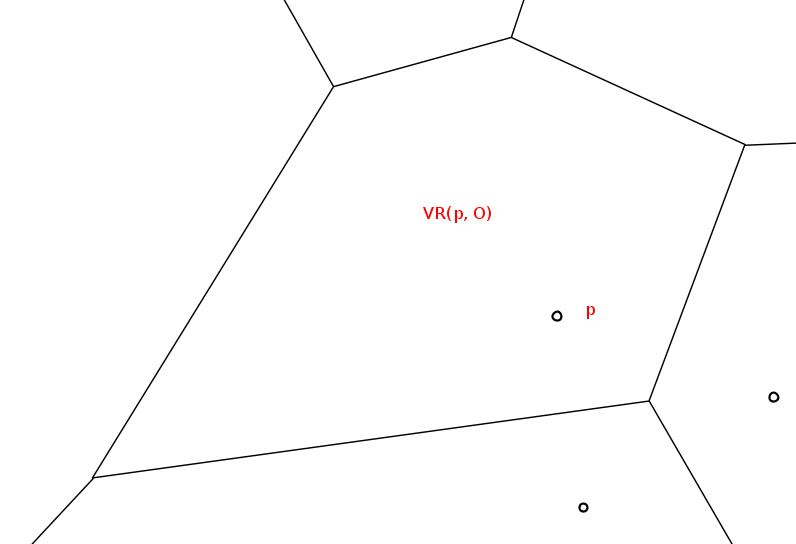
\includegraphics[width=150px]{images/voronoi_region_example_01.png}
\caption{Beispiel einer Voronoi-Region: $VR(p, O)$, ausgehend vom Punkt $p$\protect\footnotemark}
\label{fig:voronoiRegionExample01}
\end{figure}
\footnotetext{Eigene Darstellung}


Entfernt man nun sämtliche Voronoi-Regionen aus der Ebene, bleiben genau die Punkte des Raumes $\mathbb{R}^2$ übrig, die keinen eindeutigen, sondern zwei oder mehr nächste Nachbarn in der Objekt-Menge $O$ besitzen. Diese Punktemenge ist das \textbf{Voronoi-Diagramm} $\bm{V(O)}$ von $O$~\parencite[S. 212]{klein2005algorithmischegeometrie}.

\begin{figure}[h]
\centering
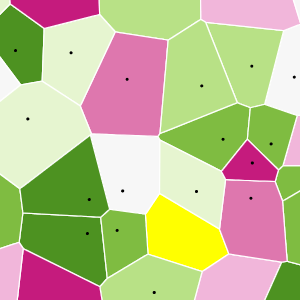
\includegraphics[width=120px]{images/voronoi_example_01.png}
\caption{Beispiel eines Voronoi-Diagramms\protect\footnotemark}
\label{fig:voronoiExample01}
\end{figure}
\footnotetext{\cite{mbostock2012}}

\newpage{}

Ein gemeinsames Randstück von zwei Voronoi-Regionen wird als \textbf{Voronoi-Kante} bezeichnet, die Ecken einer Voronoi-Region werden als \textbf{Voronoi-Knoten} bezeichnet~\parencite[S. 213]{klein2005algorithmischegeometrie}.

\begin{figure}[h]
\centering
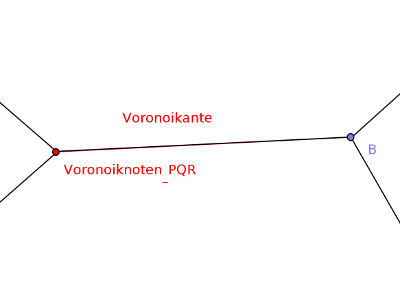
\includegraphics[width=200px]{images/voronoi_kante_knoten.png}
\caption{Beispiel einer Voronoi-Kante und eines Voronoi-Knotens\protect\footnotemark}
\label{fig:voronoiEdgeKnot}
\end{figure}
\footnotetext{Eigene Darstellung mittels Geogebra}

Liegt ein Punkt $p$ der Punktemenge $O$ auf deren \glslink{convexHull}{konvexer Hülle}, so hat der Punkt eine unbeschränkte Voronoi-Region~\parencite[S. 217]{klein2005algorithmischegeometrie}.

Was passiert nun aber, wenn Punkte aus der Menge $O$ beispielsweise auf einer gemeinsamen Geraden liegen? Dies führt zu dem Problem, dass ein nicht-zusammenhängendes Voronoi-Diagramm entsteht. \citeauthor{klein2005algorithmischegeometrie} schlägt vor, dass der ``interessante'' Teil des Diagramms von einem einfachen geschlossenen Weg $\Gamma$ umschlossen wird, der so weit aussen verläuft, dass er nur unbeschränkte Voronoi-Kanten kreuzt, welche dort abgeschnitten werden~\parencite[S. 217]{klein2005algorithmischegeometrie}.

Aus den genannten Punkten lassen sich gemäss~\citeauthor{klein2005algorithmischegeometrie} einige interssante Eigenschaften ableiten:
\begin{compactitem}
\item ``Das Voronoi-Diagramm von $n$ Punkten in der Ebene hat $O(n)$ viele Knoten und Kanten. Der Rand einer Voronoi-Region besteht im Mittel aus höchstens sechs Kanten.'' (\citeyear{klein2005algorithmischegeometrie}, S. 219)
\item ``Aus dem Voronoi-Diagramm $V(S)$ einer $n$-elementigen Punktemenge $S$ lässt sich in Zeit $O(n)$ die konvexe Hülle von $S$ ableiten.'' (ebd.)
\item ``Das Voronoi-Diagramm von $n$ Punkten in der Ebene zu konstruieren hat die Zeitkomplexität $\Omega(n \log{n})$.'' (ebd.)
\end{compactitem}
